% Generated by render.py; edit preamble.tex, citations.json and main.tikz
\documentclass[border=12pt]{standalone}
\def\pgfsysdriver{pgfsys-dvisvgm.def}
\usepackage[dvisvgm]{xcolor}
\usepackage{xeCJK}
\setCJKmainfont{HaranoAjiGothic-Regular.otf}[BoldFont=HaranoAjiGothic-Bold.otf]
\setCJKsansfont{HaranoAjiGothic-Regular.otf}[BoldFont=HaranoAjiGothic-Bold.otf]
\usepackage{amsmath,amssymb,tikz,lmodern}
\usetikzlibrary{arrows.meta,positioning,calc,fit,backgrounds}
\renewcommand{\familydefault}{\sfdefault}
\definecolor{ink}{HTML}{25322F}
\definecolor{green}{HTML}{246657}
\definecolor{tint}{HTML}{EEF4F0}
\definecolor{soft}{HTML}{C6D2CC}
\definecolor{muted}{HTML}{52615B}
\newif\ifJapanese
\newcommand{\Tx}[2]{\ifJapanese #1\else #2\fi}
\newcommand{\Eff}{\overline{\operatorname{Eff}}}
\newcommand{\heading}[3]{{\color{green}\bfseries #1\quad\Tx{#2}{#3}}\\[5pt]}
% A white rectangle makes the complete citation label clickable, including spaces.
\newcommand{\refurl}[2]{\special{dvisvgm:raw <a xlink:href="#1" target="_blank" rel="noopener noreferrer">}{\setlength{\fboxsep}{0pt}\colorbox{white}{\color{green}\underline{\strut #2}}}\special{dvisvgm:raw </a>}}
\tikzset{
 card/.style={draw=soft,fill=white,rounded corners=2pt,align=left,text=ink,font=\fontsize{10.5}{14}\selectfont,inner xsep=12pt,inner ysep=10pt,text width=14.4cm},
 half/.style={card,text width=6.45cm,minimum height=2.05cm},
 result/.style={card,draw=green,fill=tint,line width=.9pt},
 reason/.style={align=left,text=muted,font=\fontsize{9}{12}\selectfont,inner sep=0pt,text width=12.6cm},
 branchreason/.style={reason,text width=5.95cm},
 edge/.style={-{Stealth[length=2.4mm]},draw=green,line width=1pt},
 wire/.style={draw=green,line width=1pt},
}
% Keep the arrow in a dedicated left gutter; explanations never cover it.
\def\flow#1#2#3;{
 \coordinate (#2-from) at ($(#1.south)+(-6.9,0)$);
 \coordinate (#2-to) at ($(#2.north)+(-6.9,0)$);
 \draw[edge] (#2-from)--(#2-to);
 \node[reason,anchor=west] (#2-reason) at ($(#2-from)!.5!(#2-to)+(.55,0)$) {#3};
}

% Style adapted from the repository's Schnell diagrams; MIT attribution retained.

% Generated from citations.json; do not edit.
\newcommand{\Cite}[1]{\csname cite-#1\endcsname}
\expandafter\def\csname cite-main-result\endcsname{\shortstack[l]{\refurl{https://github.com/openai/math/blob/1581d4cbdd69a0faf34b2089614fe2a814316a6a/preprints/Uniform-exclusion-of-Landau-Siegel-zeros-October-1-2026/paper.pdf}{Theorem 1 · p. 1}}}
\expandafter\def\csname cite-prime-bias\endcsname{\shortstack[l]{\refurl{https://github.com/openai/math/blob/1581d4cbdd69a0faf34b2089614fe2a814316a6a/preprints/Uniform-exclusion-of-Landau-Siegel-zeros-October-1-2026/paper.pdf}{Lemma 2; (2.3)–(2.4) · pp. 2–3}}}
\expandafter\def\csname cite-interpolation\endcsname{\shortstack[l]{\refurl{https://github.com/openai/math/blob/1581d4cbdd69a0faf34b2089614fe2a814316a6a/preprints/Uniform-exclusion-of-Landau-Siegel-zeros-October-1-2026/paper.pdf}{Lemma 3 · p. 3}}}
\expandafter\def\csname cite-interpolation-proof\endcsname{\shortstack[l]{\refurl{https://github.com/openai/math/blob/1581d4cbdd69a0faf34b2089614fe2a814316a6a/preprints/Uniform-exclusion-of-Landau-Siegel-zeros-October-1-2026/paper.pdf}{§3, proof of Lemma 3; Corollary 4 · pp. 3–5}}}
\expandafter\def\csname cite-determinant\endcsname{\shortstack[l]{\refurl{https://github.com/openai/math/blob/1581d4cbdd69a0faf34b2089614fe2a814316a6a/preprints/Uniform-exclusion-of-Landau-Siegel-zeros-October-1-2026/paper.pdf}{§4; Lemma 6 · pp. 5–6}}}
\expandafter\def\csname cite-divisibility\endcsname{\shortstack[l]{\refurl{https://github.com/openai/math/blob/1581d4cbdd69a0faf34b2089614fe2a814316a6a/preprints/Uniform-exclusion-of-Landau-Siegel-zeros-October-1-2026/paper.pdf}{Lemma 7; (5.2)–(5.6) · p. 7}}}
\expandafter\def\csname cite-norm-bounds\endcsname{\shortstack[l]{\refurl{https://github.com/openai/math/blob/1581d4cbdd69a0faf34b2089614fe2a814316a6a/preprints/Uniform-exclusion-of-Landau-Siegel-zeros-October-1-2026/paper.pdf}{(5.1), (5.7) · pp. 7–8}}}
\expandafter\def\csname cite-completion\endcsname{\shortstack[l]{\refurl{https://github.com/openai/math/blob/1581d4cbdd69a0faf34b2089614fe2a814316a6a/preprints/Uniform-exclusion-of-Landau-Siegel-zeros-October-1-2026/paper.pdf}{§6; (6.1)–(6.2) · p. 8}}}
\expandafter\def\csname cite-log-derivative\endcsname{\shortstack[l]{\refurl{https://page-one.springer.com/pdf/preview/10.1007/978-1-4757-5927-3_14}{[D80, §14, (2), 誌面 p. 89 / PDF p. 2]}}}

\Japanesetrue
\begin{document}
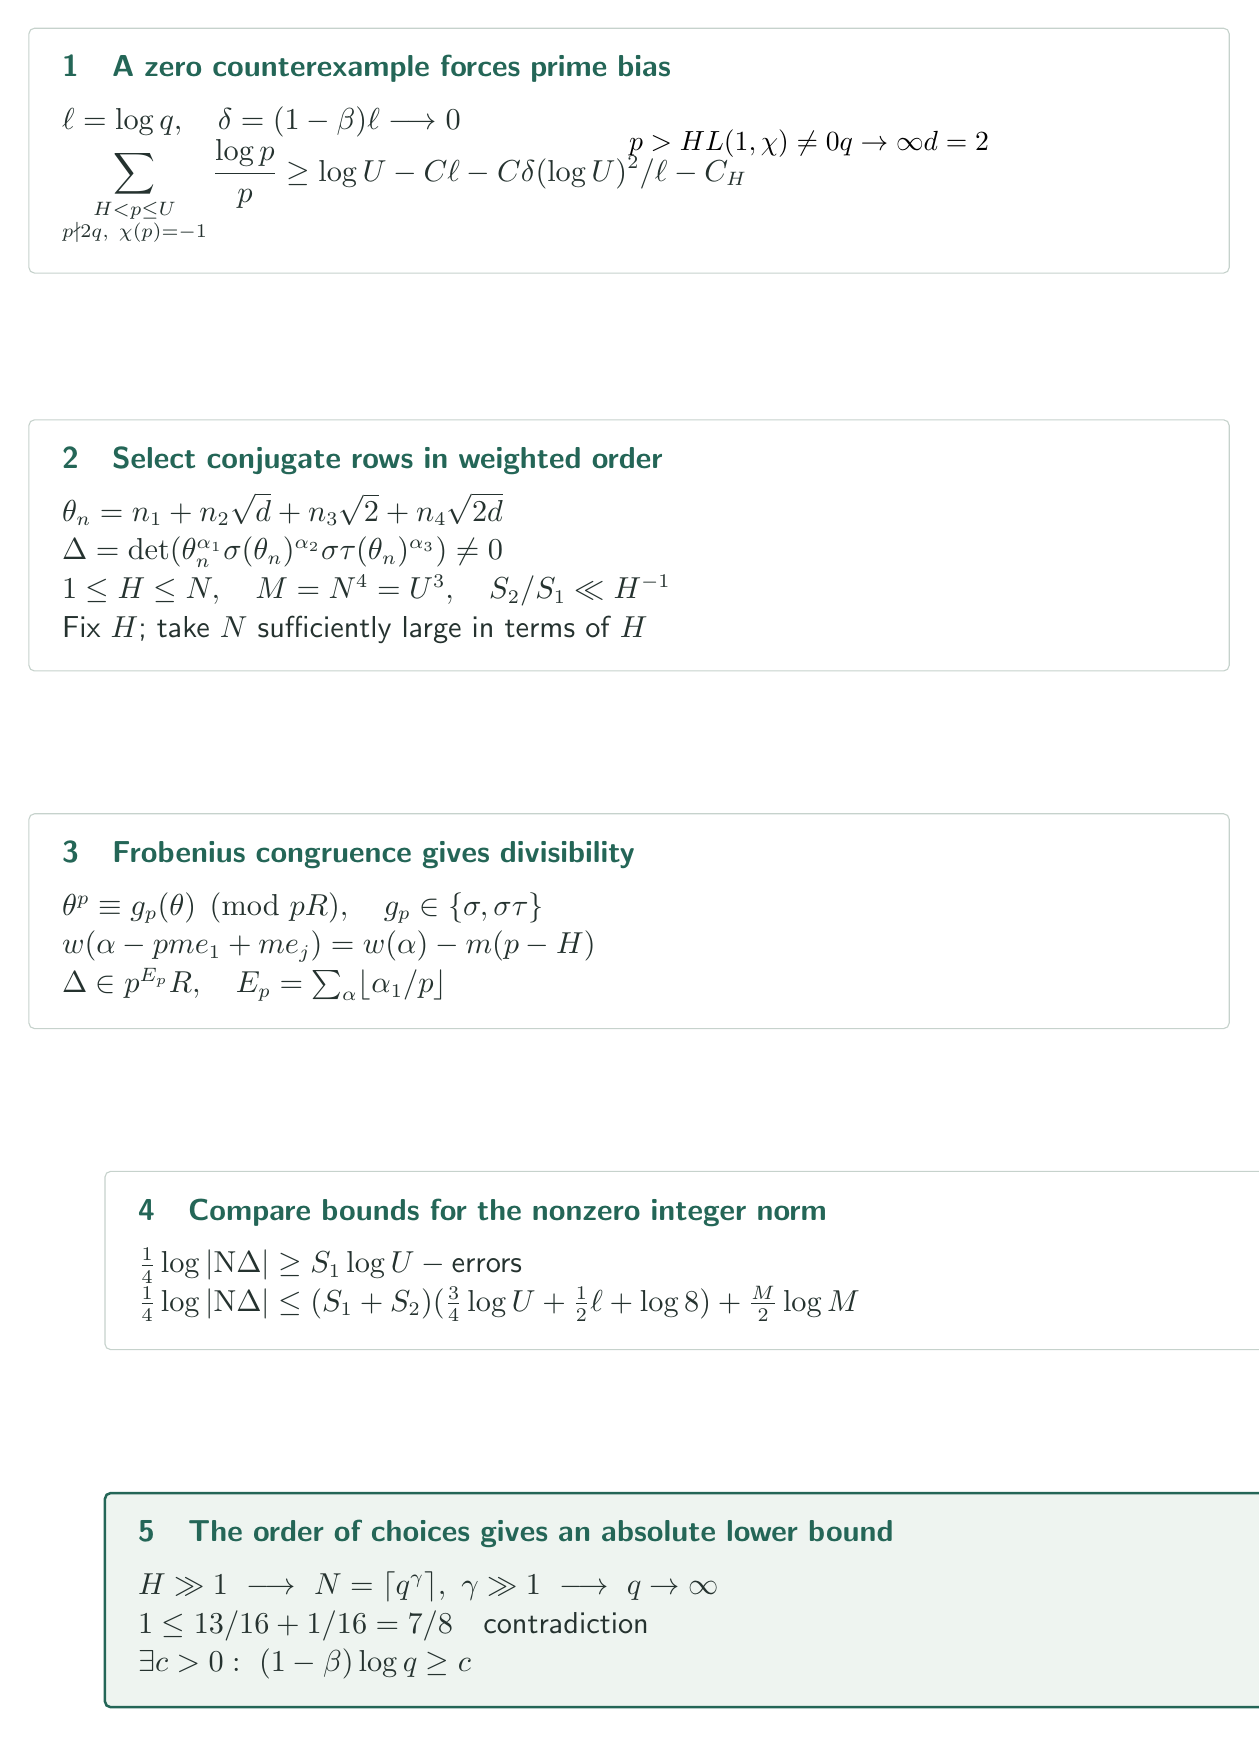
\begin{tikzpicture}
\node[card] (a) {\heading{1}{零点の反例列を素数の偏りへ}{A zero counterexample forces prime bias}
$\ell=\log q,\quad\delta=(1-\beta)\ell\longrightarrow0$\\
$\displaystyle\sum_{\substack{H<p\le U\\p\nmid2q,\ \chi(p)=-1}}\frac{\log p}{p}
\ge\log U-C\ell-C\delta(\log U)^2/\ell-C_H$};
\node[card,below=1.85cm of a] (b) {\heading{2}{共役の行を重み順に選ぶ}{Select conjugate rows in weighted order}
$\theta_n=n_1+n_2\sqrt d+n_3\sqrt2+n_4\sqrt{2d}$\\
$\Delta=\det(\theta_n^{\alpha_1}\sigma(\theta_n)^{\alpha_2}\sigma\tau(\theta_n)^{\alpha_3})\ne0$\\
$1\le H\le N,\quad M=N^4=U^3,\quad S_2/S_1\ll H^{-1}$\\
\Tx{$H$ 固定、$N$ は $H$ に対し十分大}{Fix $H$; take $N$ sufficiently large in terms of $H$}};
\flow{a}{b}{\Tx{素数和と独立に補間を準備し、後で二つを合流させる}{Prepare interpolation independently, then combine the two inputs}\\\Cite{prime-bias}\quad\Cite{log-derivative}\\\Cite{interpolation}\quad\Cite{determinant}};
\node[card,below=1.8cm of b] (c) {\heading{3}{Frobenius合同式が可除性を与える}{Frobenius congruence gives divisibility}
$\theta^p\equiv g_p(\theta)\pmod{pR},\quad g_p\in\{\sigma,\sigma\tau\}$\\
$w(\alpha-pme_1+me_j)=w(\alpha)-m(p-H)$\\
$\Delta\in p^{E_p}R,\quad E_p=\sum_{\alpha}\lfloor\alpha_1/p\rfloor$};
\flow{b}{c}{\Tx{$p>H$ なら補正行は先行行の張る空間に入り、行列式は不変}{For $p>H$, corrections lie in the earlier span and preserve the determinant}\\\Cite{divisibility}};
\node[card,below=1.8cm of c] (d) {\heading{4}{非零整数ノルムの上下界を比較}{Compare bounds for the nonzero integer norm}
$\tfrac14\log|\mathrm N\Delta|\ge S_1\log U-\text{\Tx{誤差}{errors}}$\\
$\tfrac14\log|\mathrm N\Delta|\le(S_1+S_2)(\tfrac34\log U+\tfrac12\ell+\log8)+\tfrac M2\log M$};
\flow{c}{d}{\Tx{素数の対数質量を合算し、複素埋込みでHadamard上界を得る}{Sum logarithmic prime mass and apply Hadamard at all complex embeddings}\\\Cite{norm-bounds}};
\node[result,below=1.8cm of d] (e) {\heading{5}{固定する順序が絶対的な下限を与える}{The order of choices gives an absolute lower bound}
$H\gg1\ \longrightarrow\ N=\lceil q^\gamma\rceil,\ \gamma\gg1\ \longrightarrow\ q\to\infty$\\
$1\le13/16+1/16=7/8\quad\text{\Tx{矛盾}{contradiction}}$\\
$\exists c>0:\ (1-\beta)\log q\ge c$};
\flow{d}{e}{\Tx{$L(1,\chi)\ne0$ で $q\to\infty$ とし、固定例外 $d=2$ を除く}{Use $L(1,\chi)\ne0$ to force $q\to\infty$ and remove the fixed exception $d=2$}\\\Cite{completion}};

\end{tikzpicture}
\end{document}
